\documentclass[letterpaper,twocolumn,openany,nodeprecatedcode]{article}

\usepackage[english]{babel}

\usepackage[utf8]{inputenc}
\usepackage[singlelinecheck=false]{caption}
\usepackage{lipsum}
\usepackage{listings}
\usepackage{shortvrb}
\usepackage{stfloats}
\usepackage[table]{xcolor}
\usepackage{tikz}
%\usepackage{sectsty}
%\usepackage[sfdefault,condensed]{cabin}
\usepackage{fontspec}
\usetikzlibrary{shapes}
\usepackage{titlesec}
%\usepackage[T1]{fontenc}
\setmainfont{Interstate Condensed}
\newfontfamily\sectionfont{Brokenscript-BoldCond}
\titleformat*{\section}{\Large\bfseries\sectionfont}
\titleformat*{\subsection}{\large\bfseries\sectionfont}
\titleformat*{\subsubsection}{\sectionfont}
\usetikzlibrary{mindmap,trees,shadows,decorations.pathmorphing}

\MakeShortVerb{|}

\lstset{%
  basicstyle=\ttfamily,
  language=[LaTeX]{TeX},
  breaklines=true,
}

\title{Mausritter tex template}
\author{Adam Saleh}
\date{2020/04/21}

\begin{document}


\section{Make a mouse}

The world is very big and very dangerous for a small
mouse adventurer. You will need to be very brave, and
always keep your wits about you.

\subsection{Attributes}

Your mouse has three attributes. These measure their
basic strengths and weaknesses.

\begin{itemize}
  \item \textbf{STR}: physical disposition
  \item \textbf{DEX}: speed and agility
  \item \textbf{WIL}: strenght of will and charisma
\end{itemize}

\subsection{HP, pips and background}

{\rowcolors{1}{gray!60}{white}
\begin{tabular}{ c c c  }
d6 & Sign & Disposition \\
\hline
1 & AF & AFG \\
2 & AX   & ALA \\
3 & ALB \\
4 & DZA \\
5 & AS & ASM \\
6 & AD & AND   \\
\end{tabular}
}

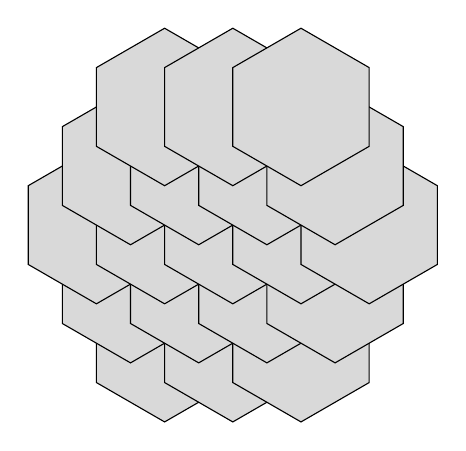
\begin{tikzpicture} [hexa/.style= {shape=regular polygon,regular polygon sides=6,minimum size=2cm, draw,inner sep=0,anchor=south,fill=white!85!black,rotate=30}]

\foreach \j in {0,...,1}{%
\pgfmathsetmacro\end{2+\j}
  \foreach \i in {0,...,\end}{%
  \node[hexa] (h\i;\j) at ({(\i-\j/2)*sin(60)},{\j*0.75}) {};}  }
\foreach \j in {0,...,2}{%
  \pgfmathsetmacro\end{4-\j}
  \foreach \i in {0,...,\end}{%
  \pgfmathtruncatemacro\k{\j+6}
  \node[hexa] (h\i;\k) at ({(\i+\j/2-1)*sin(60)},{1.5+\j*0.75}) {};}  }

%  \foreach \k in {0,...,10}  {\node [circle,red,minimum size=1cm] at (h3;\k) {3;\k};}
%   \foreach \k in {0,...,10}  {\node [circle,blue,minimum size=1cm] at (h1;\k) {1;\k};}
\end{tikzpicture}

\end{document}
